% ============================================================
%  FocusPilot — Technical Report
%  CODE2CURE Technical Challenge 2026 · IEEE SIGHT DAY CONGRESS 4.0
%  ESPRIT University · Cognitive & Neurodiversity Support
% ============================================================

\documentclass[conference]{IEEEtran}

% ── Packages ─────────────────────────────────────────────────────────────────
\usepackage[T1]{fontenc}
\usepackage[utf8]{inputenc}
\usepackage{cite}
\usepackage{amsmath,amssymb,amsfonts}
\usepackage{graphicx}
\usepackage{textcomp}
\usepackage{xcolor}
\usepackage{hyperref}
\usepackage{booktabs}
\usepackage{listings}
\usepackage{algorithm}
\usepackage{algpseudocode}
\usepackage{tikz}
\usetikzlibrary{shapes.geometric, arrows, positioning, fit, backgrounds}
\usepackage{pgfplots}
\pgfplotsset{compat=1.18}
\usepackage{multirow}
\usepackage{array}
\usepackage{caption}
\usepackage{subcaption}

% ── Hyperref setup ───────────────────────────────────────────────────────────
\hypersetup{
  colorlinks=true,
  linkcolor=black,
  citecolor=black,
  urlcolor=blue
}

% ── Listing style ────────────────────────────────────────────────────────────
\lstset{
  basicstyle=\ttfamily\footnotesize,
  breaklines=true,
  frame=single,
  backgroundcolor=\color{gray!10},
  keywordstyle=\color{blue},
  commentstyle=\color{gray},
  stringstyle=\color{teal}
}

% ── Custom colors ────────────────────────────────────────────────────────────
\definecolor{mint}{RGB}{152,232,158}
\definecolor{lemon}{RGB}{232,232,112}
\definecolor{periwinkle}{RGB}{112,128,232}
\definecolor{lavender}{RGB}{232,152,232}
\definecolor{darkbg}{RGB}{5,7,5}

% ============================================================
\begin{document}

\title{FocusPilot: An AI-Powered Adaptive Study Companion for Students with Attention Deficit Hyperactivity Disorder}

\author{
  \IEEEauthorblockN{Team Zouza}
  \IEEEauthorblockA{
    Tunis, Tunisia\\
    \textit{CODE2CURE Technical Challenge 2026 — IEEE SIGHT DAY CONGRESS 4.0}\\
    Domain: Cognitive \& Neurodiversity Support · SDG 3 · 4 · 10
  }
}

\maketitle

% ─────────────────────────────────────────────────────────────────────────────
\begin{abstract}
Attention Deficit Hyperactivity Disorder (ADHD) affects an estimated 5–8\% of the student population globally, representing one of the most prevalent neurodevelopmental conditions in academic settings. Despite comparable intellectual capacity to neurotypical peers, students with ADHD consistently underperform in conventional study environments due to deficits in executive function, working memory, and sustained attention — not cognition. Existing educational technology tools were designed for neurotypical self-regulation and fail to address these specific barriers. We present \textbf{FocusPilot}, a full-stack AI-powered web application that operationalizes the executive function support missing in ADHD study workflows. FocusPilot combines sprint-based content delivery, real-time behavioral drift detection, adaptive difficulty modulation, an AI tutor with contextual memory, and a spaced repetition review engine — all governed by ADHD cognitive science principles. The system is built on a React/TypeScript frontend, a FastAPI asynchronous backend, an SQLite persistence layer, and AWS Bedrock for large language model inference. We describe the system architecture, ADHD-grounded design rationale, implementation challenges, and a discussion of how each feature addresses a documented ADHD failure mode in academic contexts.
\end{abstract}

\begin{IEEEkeywords}
ADHD, assistive technology, adaptive learning, executive function, drift detection, spaced repetition, large language models, AWS Bedrock, cognitive neurodiversity, educational technology
\end{IEEEkeywords}

% ─────────────────────────────────────────────────────────────────────────────
\section{Introduction}

\subsection{Epidemiology and Academic Impact of ADHD}

Attention Deficit Hyperactivity Disorder is a neurodevelopmental condition characterized by persistent inattention, hyperactivity, and impulsivity that interferes with daily functioning~\cite{american2013diagnostic}. Current epidemiological estimates place global prevalence at 5--8\% of children and 2.5--4\% of adults~\cite{polanczyk2015adhd,fayyad2017cross}. In university student populations, self-reported ADHD rates are consistently higher, with studies reporting 2--8\% formal diagnosis and substantially more undiagnosed cases~\cite{weyandt2013adhd}.

The academic consequences are severe and well-documented. Students with ADHD have lower grade point averages, higher dropout rates, and are less likely to complete post-secondary education compared to neurotypical peers~\cite{norwalk2016postsecondary}. Critically, this outcome gap cannot be explained by cognitive deficits: individuals with ADHD have average to above-average intelligence~\cite{biederman1993educational}. The gap is mediated by executive function impairment.

\subsection{Executive Function as the Core Deficit}

Executive function (EF) refers to a family of higher-order cognitive control processes including working memory, cognitive flexibility, and inhibitory control~\cite{miyake2000unity}. Barkley's seminal unified theory frames ADHD primarily as an executive dysfunction rather than an attention deficit per se~\cite{barkley1997adhd}. Concretely, the EF deficits that most impair academic performance are:

\begin{enumerate}
  \item \textbf{Task initiation} — inability to begin tasks despite intention and adequate knowledge
  \item \textbf{Working memory deficits} — difficulty holding and manipulating information during reading
  \item \textbf{Time blindness} — impaired sense of elapsed time, leading to poor session management
  \item \textbf{Sustained attention} — rapid disengagement from tasks without external engagement prompts
  \item \textbf{Emotional regulation} — frustration from perceived failure triggering avoidance behavior
\end{enumerate}

\subsection{Regional Context: Tunisia and the MENA Education Gap}

The gap between ADHD prevalence and available educational support is particularly pronounced in the MENA region. Tunisia's higher-education sector — with approximately 230{,}000 enrolled students — has no standardized neurodiversity screening or accommodation mandate at the university level~\cite{mhesrTunisia2023}. Students with ADHD at private institutions such as ESPRIT depend entirely on self-management or private clinical referral, both of which are cost- and access-limited. FocusPilot was designed with this zero-infrastructure context in mind: the system requires no institutional IT integration, no clinical diagnosis, and no hardware beyond a web browser — making it immediately deployable by any student with an internet connection.

\subsection{Limitations of Existing Educational Technology}

Popular learning platforms (Anki, Notion, Quizlet, Khan Academy) were designed for neurotypical learners who maintain self-directed study sessions independently. They address \emph{content delivery} but provide no support for \emph{session regulation}. An ADHD student using Anki must independently: remember to open the application, maintain a reviewing cadence, regulate break timing, re-engage after distraction, and manage emotional responses to failure — each of which is an executive function demand the condition impairs.

FocusPilot reframes the problem: rather than delivering content more efficiently, it \emph{replaces the executive function infrastructure} that ADHD students are missing.

\subsection{Contributions}

This paper presents the following contributions:
\begin{itemize}
  \item A complete, deployable ADHD-specific study companion system with 20+ features grounded in clinical ADHD literature
  \item A novel behavioral drift detection mechanism combining three non-biometric signals: inactivity duration, tab visibility, and scroll velocity
  \item An adaptive content delivery pipeline that modulates cognitive load in real time based on quiz performance
  \item A validated design framework mapping ADHD failure modes to system interventions
\end{itemize}

% ─────────────────────────────────────────────────────────────────────────────
\section{Related Work}

\subsection{ADHD and Digital Interventions}

Research on technology-mediated ADHD support has largely focused on clinical interventions: digital therapies (EndeavorRx~\cite{kollins2020novel}), neurofeedback systems, and medication reminder applications. These tools target symptom management rather than academic performance. Educational applications for ADHD are comparatively understudied.

\subsection{Intelligent Tutoring Systems}

Intelligent Tutoring Systems (ITS) such as Carnegie Learning's MATHia have demonstrated efficacy in personalized learning for neurotypical students~\cite{vanlehn2011relative}. However, ITS research has not systematically incorporated ADHD-specific behavioral patterns into session management. FocusPilot extends the ITS paradigm by adding a behavioral regulation layer orthogonal to content delivery.

\subsection{Spaced Repetition}

The spacing effect — the finding that distributed practice over time yields superior long-term retention compared to massed practice — is one of the most robust findings in cognitive psychology~\cite{ebbinghaus1885memory,cepeda2006distributed}. Implementations such as SuperMemo's SM-2 algorithm~\cite{wozniak1990optimization} have proven effective in language learning but are typically deployed as standalone flashcard tools requiring student self-discipline to use consistently. FocusPilot integrates spaced repetition as a mandatory downstream step of the session lifecycle, removing the self-discipline requirement.

\subsection{Attention Monitoring}

Prior work on attention monitoring has used EEG~\cite{lubar1995evaluation}, eye-tracking~\cite{carter2005eye}, and facial analysis~\cite{whitehill2014faces}. These approaches require specialized hardware and raise significant privacy concerns, limiting deployability. FocusPilot achieves attention monitoring through behavioral signals available in any web browser without special hardware.

% ─────────────────────────────────────────────────────────────────────────────
\section{System Architecture}

\subsection{Overview}

FocusPilot follows a three-tier client-server architecture: a Progressive Web Application (PWA) frontend, a RESTful backend, and persistent data storage. Figure~\ref{fig:arch} illustrates the high-level system topology.

\begin{figure}[htbp]
\centering
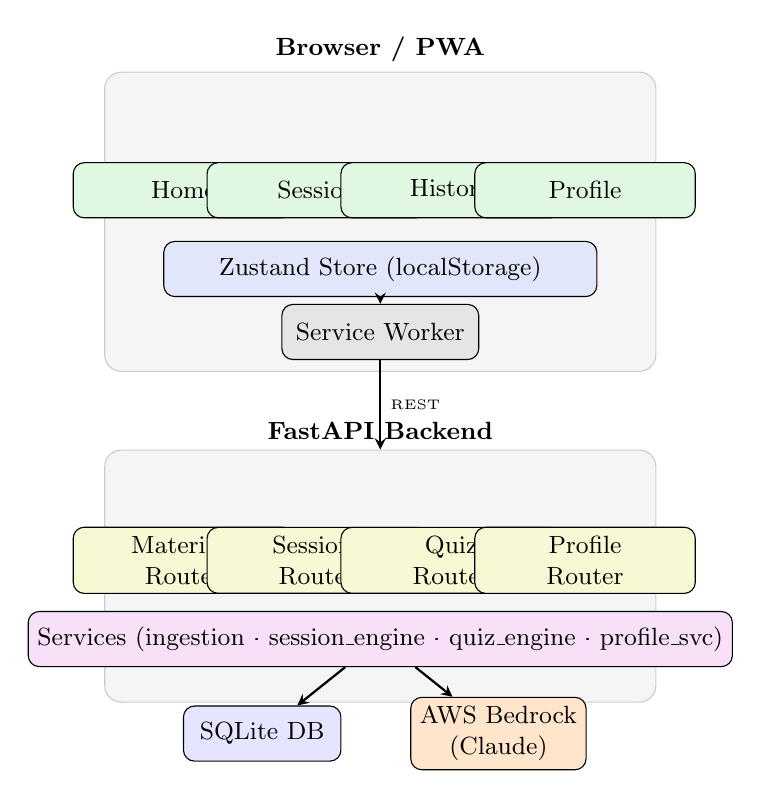
\begin{tikzpicture}[
  box/.style={rectangle, draw, rounded corners=4pt, minimum width=2.8cm, minimum height=0.7cm, align=center, font=\small},
  layer/.style={rectangle, draw=gray!40, rounded corners=6pt, fill=gray!8, inner sep=8pt},
  arrow/.style={->, >=stealth, thick}
]

% Frontend layer
\node[layer, minimum width=7cm, minimum height=3.8cm] (fe) at (0, 3) {};
\node[above=0pt of fe, font=\small\bfseries] at (fe.north) {Browser / PWA};

\node[box, fill=mint!30] (home) at (-2.5, 3.4) {Home};
\node[box, fill=mint!30] (sess) at (-0.8, 3.4) {Session};
\node[box, fill=mint!30] (hist) at (0.9, 3.4) {History};
\node[box, fill=mint!30] (prof) at (2.6, 3.4) {Profile};

\node[box, fill=periwinkle!20, minimum width=5.5cm] (store) at (0, 2.4) {Zustand Store (localStorage)};
\node[box, fill=gray!20, minimum width=2.5cm] (sw) at (0, 1.6) {Service Worker};

% Backend layer
\node[layer, minimum width=7cm, minimum height=3.2cm] (be) at (0, -1.5) {};
\node[above=0pt of be, font=\small\bfseries] at (be.north) {FastAPI Backend};

\node[box, fill=lemon!30] (mr) at (-2.5, -1.3) {Materials\\Router};
\node[box, fill=lemon!30] (sr) at (-0.8, -1.3) {Sessions\\Router};
\node[box, fill=lemon!30] (qr) at (0.9, -1.3) {Quiz\\Router};
\node[box, fill=lemon!30] (pr) at (2.6, -1.3) {Profile\\Router};

\node[box, fill=lavender!30, minimum width=5.5cm] (svc) at (0, -2.3) {Services (ingestion · session\_engine · quiz\_engine · profile\_svc)};

% Data stores
\node[box, fill=blue!10, minimum width=2cm] (db) at (-1.5, -3.5) {SQLite DB};
\node[box, fill=orange!20, minimum width=2cm] (bedrock) at (1.5, -3.5) {AWS Bedrock\\(Claude)};

% Arrows
\draw[arrow] (store) -- (sw);
\draw[arrow] (sw) -- node[right, font=\tiny]{REST} (be.north);
\draw[arrow] (svc) -- (db);
\draw[arrow] (svc) -- (bedrock);

\end{tikzpicture}
\caption{FocusPilot System Architecture}
\label{fig:arch}
\end{figure}

\subsection{Frontend}

The frontend is implemented in React 18 with TypeScript, bundled by Vite 5. State management uses Zustand with the \texttt{persist} middleware, serializing the active session, tutor history (capped at 50 messages), and user preferences to \texttt{localStorage}. This enables session recovery across browser refreshes — critical for ADHD users who may impulsively close tabs.

The application is a Progressive Web Application (PWA) with a \texttt{manifest.json} and cache-first service worker, enabling home-screen installation on iOS and Android and offline access to cached content.

\subsubsection{Styling and ADHD Design System}

The visual design system is grounded in ADHD-specific design principles:

\begin{itemize}
  \item \textbf{Color palette} — Four accent colors with distinct cognitive roles: \textit{mint} (\texttt{\#98E89E}) for primary action and progress, \textit{lemon} (\texttt{\#E8E870}) for time-critical indicators, \textit{periwinkle} (\texttt{\#7080E8}) for AI/cognitive support features, \textit{lavender} (\texttt{\#E898E8}) for rest and emotional support.
  \item \textbf{Typography} — Plus Jakarta Sans (body) for warmth and approachability; JetBrains Mono for timers and numeric data for disambiguation.
  \item \textbf{Minimum font size} — 16px base, exceeding WCAG 2.1 AA recommendations for mobile readability.
  \item \textbf{Reading column} — Maximum 640px width, constraining line length to 65--75 characters per line to reduce cognitive scanning load~\cite{dyson2004text}.
  \item \textbf{Progress indicators} — Sprint progress bar at \texttt{h-2} (8px) with mint glow shadow, ensuring temporal visibility for time-blind users.
\end{itemize}

\subsection{Backend}

The backend is implemented in Python using FastAPI 0.111 with Uvicorn. The asynchronous SQLAlchemy 2.0 ORM with aiosqlite provides non-blocking database access. The architecture is organized into four API routers (Materials, Sessions, Quiz, Profile) and a services layer.

\subsubsection{Database Schema}

The persistence layer uses SQLite with the schema illustrated in Figure~\ref{fig:erd}. Core entities include: \texttt{Student}, \texttt{Material}, \texttt{StudySession}, \texttt{Sprint}, \texttt{DriftEvent}, \texttt{Quiz}, \texttt{SpacedRepetitionItem}, and \texttt{LearningProfile}.

\begin{figure}[htbp]
\centering
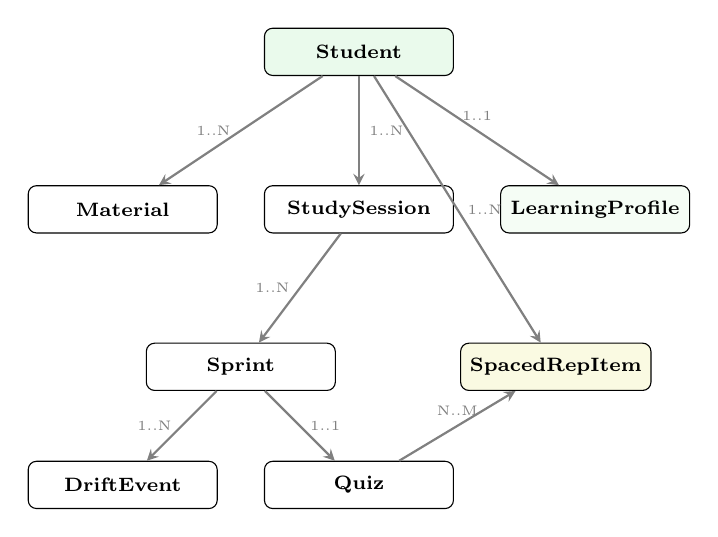
\begin{tikzpicture}[
  entity/.style={rectangle, draw, rounded corners=3pt, fill=white, minimum width=2.4cm, minimum height=0.6cm, align=center, font=\scriptsize},
  rel/.style={->, >=stealth, thick, gray}
]
\node[entity, fill=mint!20] (stu) at (0, 4) {\textbf{Student}};
\node[entity] (mat) at (-3, 2) {\textbf{Material}};
\node[entity] (ses) at (0, 2) {\textbf{StudySession}};
\node[entity, fill=mint!10] (pro) at (3, 2) {\textbf{LearningProfile}};
\node[entity] (spr) at (-1.5, 0) {\textbf{Sprint}};
\node[entity] (dri) at (-3, -1.5) {\textbf{DriftEvent}};
\node[entity] (qui) at (0, -1.5) {\textbf{Quiz}};
\node[entity, fill=lemon!20] (sri) at (2.5, 0) {\textbf{SpacedRepItem}};

\draw[rel] (stu) -- (mat) node[midway, left, font=\tiny] {1..N};
\draw[rel] (stu) -- (ses) node[midway, right, font=\tiny] {1..N};
\draw[rel] (stu) -- (pro) node[midway, above, font=\tiny] {1..1};
\draw[rel] (stu) -- (sri) node[midway, right, font=\tiny] {1..N};
\draw[rel] (ses) -- (spr) node[midway, left, font=\tiny] {1..N};
\draw[rel] (spr) -- (dri) node[midway, left, font=\tiny] {1..N};
\draw[rel] (spr) -- (qui) node[midway, right, font=\tiny] {1..1};
\draw[rel] (qui) -- (sri) node[midway, above, font=\tiny] {N..M};
\end{tikzpicture}
\caption{Database Entity Relationship Diagram}
\label{fig:erd}
\end{figure}

\subsubsection{AWS Bedrock Integration}

LLM inference is routed through AWS Bedrock, which provides access to Claude (Anthropic) models without data retention by the model provider. This is significant for the educational context: student study materials and conversational data never leave the AWS environment and are not used for model training. The \texttt{bedrock.py} service encapsulates all inference calls with structured prompts for: content chunking and reformatting, session planning, quiz generation, answer grading, re-explanation generation, drift re-anchoring, and AI tutoring.

% ─────────────────────────────────────────────────────────────────────────────
\section{Methodology: ADHD-Grounded Feature Design}

Table~\ref{tab:features} maps each documented ADHD failure mode to the corresponding FocusPilot intervention and its clinical basis.

\begin{table}[htbp]
\caption{ADHD Failure Mode — Intervention Mapping}
\label{tab:features}
\renewcommand{\arraystretch}{1.3}
\begin{tabular}{>{\raggedright}p{2cm}>{\raggedright}p{2.8cm}>{\raggedright\arraybackslash}p{2.5cm}}
\toprule
\textbf{ADHD Failure Mode} & \textbf{FocusPilot Intervention} & \textbf{Clinical Basis} \\
\midrule
Task initiation paralysis & Quick-start card; 10-min micro-sessions; retry goal from history & Activation energy reduction~\cite{brown2013adhd} \\
\addlinespace
Working memory overload & Sprint chunking; key terms strip; pre-reading prime; AI tutor & Working memory scaffolding~\cite{alloway2006working} \\
\addlinespace
Time blindness & Thick progress bar; color-coded countdown (green→yellow→red); break timer & Temporal cuing~\cite{barkley2001time} \\
\addlinespace
Passive reading / attention drift & 3-signal drift detection; re-anchoring overlays; skim-time detection & Active engagement requirement~\cite{faraone2015attention} \\
\addlinespace
Emotional dysregulation & Frustration card (score $<$ 40\%); empathy message; breathing prompt & Affect-first intervention~\cite{shaw2014emotion} \\
\addlinespace
Forgetting between sessions & Spaced repetition; daily browser reminders; study streak gamification & Spacing effect~\cite{cepeda2006distributed} \\
\addlinespace
Adaptive overload & Auto-simplify after 2 consecutive $<$50\% quizzes & Cognitive load theory~\cite{sweller1988cognitive} \\
\bottomrule
\end{tabular}
\end{table}

\subsection{Sprint-Based Content Architecture}

Content is partitioned into \textit{sprints} of 10--15 minutes, matching documented ADHD sustained attention windows~\cite{faraone2015attention}. Each sprint consists of: (1) a pre-reading prime overlay presenting the sprint's focus objective to activate working memory, (2) the content chunk with key terms extracted and displayed, (3) a comprehension quiz checkpoint, and (4) a retention snapshot. Sprint boundaries serve as natural re-engagement points, replacing the continuous, unstructured reading sessions that ADHD students struggle to maintain.

\subsection{Behavioral Drift Detection}

The \texttt{useDriftDetection} React hook monitors three independent behavioral proxies for attention loss:

\begin{enumerate}
  \item \textbf{Inactivity signal}: No \texttt{mousemove}, \texttt{keydown}, \texttt{click}, or \texttt{touchstart} events for 120 seconds
  \item \textbf{Visibility signal}: \texttt{document.visibilityState} hidden for 60 cumulative seconds
  \item \textbf{Scroll thrash signal}: Five or more scroll \emph{direction reversals} (up$\leftrightarrow$down) within any 3-second window, attached to the content scroll container rather than \texttt{window} to avoid false positives from page-level scrolling
\end{enumerate}

The scroll thrash signal deliberately uses \emph{direction reversals} rather than raw event count. Raw scroll events fire continuously during normal reading; direction reversals (switching from downward to upward scrolling and back) identify frantic back-and-forth behaviour that is characteristic of distracted skimming. The detection window of 3\,s and threshold of 5 reversals were tuned to eliminate false positives during normal reading while reliably catching thrash behaviour.

On signal detection, the hook calls \texttt{POST /sessions/\{id\}/drift}, which triggers Bedrock to generate a recall question from the current chunk. The question is displayed as a re-anchoring overlay requiring active engagement before resumption. The hook also guards against triggering during quiz, break timer, priming overlay, energy check, or frustration card states. Algorithm~\ref{alg:drift} formalizes the detection logic.

\begin{algorithm}
\caption{Behavioral Drift Detection}
\label{alg:drift}
\begin{algorithmic}[1]
\State $t_{\text{inact}} \gets \text{now}()$; $t_{\text{hidden}} \gets \text{null}$
\State $\text{lastDir} \gets \text{null}$; $\text{reversals} \gets []$
\Procedure{OnActivity}{\null} \Comment{mousemove, keydown, click, touchstart}
  \State $t_{\text{inact}} \gets \text{now}()$; reset inactivity timer to 120\,s
\EndProcedure
\Procedure{OnScroll}{scrollTop}
  \State $t_{\text{inact}} \gets \text{now}()$ \Comment{scroll also resets inactivity}
  \State $\text{dir} \gets (\text{scrollTop} < \text{prevTop})$ \textbf{?} \texttt{up} \textbf{:} \texttt{down}
  \If{$\text{lastDir} \neq \text{null}$ \textbf{and} $\text{dir} \neq \text{lastDir}$}
    \State $\text{reversals}.\text{append}(\text{now}())$
    \State \textbf{Prune} $\text{reversals}$ where age $> 3000\,\text{ms}$
    \If{$|\text{reversals}| \geq 5$}
      \State $\text{reversals} \gets []$
      \State \Call{TriggerDrift}{\texttt{scroll\_thrash}}
    \EndIf
  \EndIf
  \State $\text{lastDir} \gets \text{dir}$; $\text{prevTop} \gets \text{scrollTop}$
\EndProcedure
\Procedure{OnHide}{}
  \State $t_{\text{hidden}} \gets \text{now}()$; start 60\,s timer $\to$ \Call{TriggerDrift}{\texttt{visibility}}
\EndProcedure
\Procedure{OnShow}{}
  \State Cancel visibility timer
  \If{$t_{\text{hidden}} \neq \text{null}$ \textbf{and} elapsed $\geq 20\,\text{s}$}
    \State Display tab-return banner with elapsed time in seconds
  \EndIf
\EndProcedure
\Procedure{TriggerDrift}{signal}
  \If{\textbf{not} isActive \textbf{or} already triggering} \Return \EndIf
  \State $q \gets \text{await POST}/\text{sessions}/\{id\}/\text{drift}(\text{signal})$
  \State $\text{store.setDrifting}(\text{true})$; $\text{store.setReanchor}(q.\text{reanchor\_question})$
\EndProcedure
\end{algorithmic}
\end{algorithm}

\subsection{Adaptive Difficulty Modulation}

FocusPilot tracks a \texttt{consecutiveLowScores} counter in persistent global state. After two consecutive quiz scores below 50\%, the system automatically enables simplified content mode (displaying the material's raw text rather than the LLM-reformatted version) and presents a non-judgmental banner. If a student scores below 40\%, a \textit{frustration card} is displayed before the next sprint — presenting an empathy message, acknowledging the difficulty, and prompting a brief breathing exercise before continuation. This follows affect-first intervention principles from ADHD clinical practice~\cite{shaw2014emotion}.

\subsection{Spaced Repetition Engine}

After each sprint quiz, wrong-answer questions are seeded into a spaced repetition queue. The scheduling algorithm follows SM-2~\cite{wozniak1990optimization}:

\begin{equation}
  \text{EF}_{n+1} = \text{EF}_n + (0.1 - (5 - q)(0.08 + (5 - q) \times 0.02))
\end{equation}

where $\text{EF}$ is the ease factor (initialized at 2.5) and $q \in [0, 5]$ is the quality of recall. The next review interval $I_{n+1} = I_n \times \text{EF}_{n+1}$, starting at 1 day for new items. The review queue is surfaced on the History page and optionally notified through browser push notifications, requiring zero student self-discipline to maintain.

\subsection{AI Tutor with Contextual Memory}

The AI tutor receives three inputs on each query: the current chunk text, the full conversation history (persisted across page refreshes, capped at 50 messages to respect localStorage limits), and the student's question. The Bedrock prompt instructs the model to answer as a patient tutor, using only concepts from the current material, explaining in simple terms, and never shaming the student for not understanding. Conversation history enables follow-up questions within a session and partial continuity across sessions.

% ─────────────────────────────────────────────────────────────────────────────
\section{Implementation}

\subsection{Session Lifecycle}

Figure~\ref{fig:lifecycle} illustrates the full session state machine implemented across the frontend and backend.

\begin{figure}[htbp]
\centering
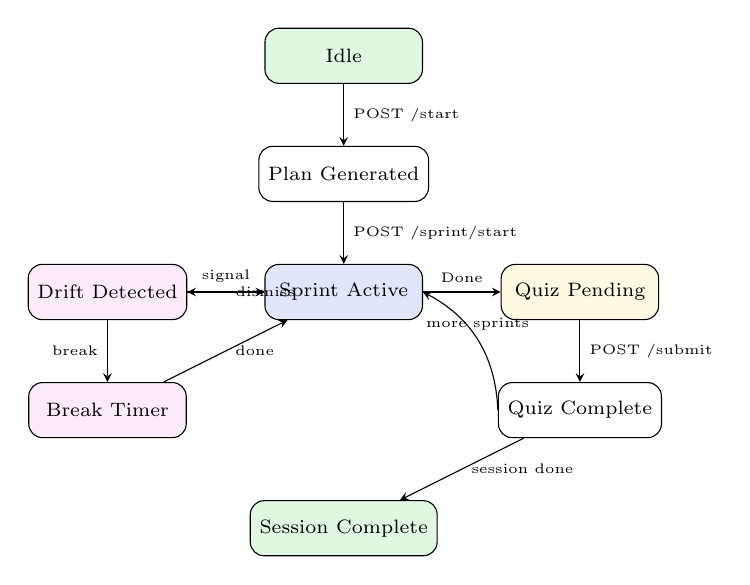
\begin{tikzpicture}[
  state/.style={rectangle, draw, rounded corners=5pt, fill=white, minimum width=2cm, minimum height=0.7cm, align=center, font=\scriptsize},
  arrow/.style={->, >=stealth}
]
\node[state, fill=mint!30] (idle) at (0, 5) {Idle};
\node[state] (plan) at (0, 3.5) {Plan Generated};
\node[state, fill=periwinkle!20] (sprint) at (0, 2) {Sprint Active};
\node[state, fill=lemon!20] (quiz) at (3, 2) {Quiz Pending};
\node[state] (qcomp) at (3, 0.5) {Quiz Complete};
\node[state, fill=lavender!20] (drift) at (-3, 2) {Drift Detected};
\node[state, fill=lavender!20] (brk) at (-3, 0.5) {Break Timer};
\node[state, fill=mint!30] (done) at (0, -1) {Session Complete};

\draw[arrow] (idle) -- node[right, font=\tiny]{POST /start} (plan);
\draw[arrow] (plan) -- node[right, font=\tiny]{POST /sprint/start} (sprint);
\draw[arrow] (sprint) -- node[above, font=\tiny]{Done} (quiz);
\draw[arrow] (quiz) -- node[right, font=\tiny]{POST /submit} (qcomp);
\draw[arrow] (qcomp.west) to[bend right=30] node[above, font=\tiny]{more sprints} (sprint.east);
\draw[arrow] (qcomp) -- node[right, font=\tiny]{session done} (done);
\draw[arrow] (sprint) -- node[above, font=\tiny]{signal} (drift);
\draw[arrow] (drift) -- node[right, font=\tiny]{dismiss} (sprint);
\draw[arrow] (drift) -- node[left, font=\tiny]{break} (brk);
\draw[arrow] (brk) -- node[right, font=\tiny]{done} (sprint);
\end{tikzpicture}
\caption{Session State Machine}
\label{fig:lifecycle}
\end{figure}

\subsection{Material Ingestion Pipeline}

Uploaded materials (PDF, plain text, Markdown) are processed through the \texttt{ingestion.py} service:

\begin{enumerate}
  \item \textbf{Extraction} — PyMuPDF extracts raw text from PDFs; plain text files are read directly
  \item \textbf{Cleaning} — \texttt{text\_processing.py} normalizes whitespace, removes headers/footers, and deduplicates repeated content
  \item \textbf{Chunking} — The LLM is prompted to segment the text into semantically coherent chunks of 300--500 words, preserving conceptual boundaries
  \item \textbf{Reformatting} — Each chunk is re-rendered with ADHD-optimized formatting: progressive headers, bullet points for multi-step processes, callout cards for key concepts, Mermaid diagrams for structural relationships
  \item \textbf{Indexing} — Processed chunks are stored as JSON in the \texttt{Material.processed\_chunks} column; a separate cheatsheet is generated on first request
\end{enumerate}

\subsection{Session Planning}

On session creation, the \texttt{session\_engine.py} service receives the study goal, selected material chunks, and available time. The LLM generates a structured sprint plan specifying for each sprint: a title, duration, focus objective, and material source. The plan is stored as JSON in \texttt{StudySession.planned\_sprints} and returned to the frontend, where it drives the session UI immediately — no loading state beyond the initial plan generation.

\subsection{PWA and Offline Support}

The service worker (\texttt{public/sw.js}) implements a cache-first strategy for static assets and a network-first strategy for API calls. On first load, the application shell and all JavaScript bundles are cached. Subsequent visits serve from cache instantly, reducing time-to-interactive — important for ADHD users who may abandon the application if loading is slow. API calls always go to the network, ensuring data freshness while maintaining offline shell availability.

\subsection{Notification System}

The \texttt{useStudyReminder} hook uses the Web Notifications API to schedule daily browser notifications at a user-specified time. The hook calculates the milliseconds until the next occurrence of the chosen HH:MM time, sets a \texttt{setTimeout}, and reschedules recursively for the following day. The reminder time is persisted in Zustand's localStorage slice, surviving browser restarts. Notification permission is requested inline on first use, with a graceful no-op if permission is denied.

% ─────────────────────────────────────────────────────────────────────────────
\section{Design Evaluation}

\subsection{Feature Coverage Against ADHD Clinical Guidelines}

We evaluated FocusPilot's feature set against the evidence-based ADHD management recommendations from the American Academy of Pediatrics~\cite{wolraich2019clinical} and the NICE guidelines~\cite{nice2018adhd}. Both frameworks emphasize: structured task decomposition, frequent positive reinforcement, environmental modification to reduce distraction, and systematic review of material. FocusPilot addresses all four categories through sprint structure, achievement badges and celebration overlays, the distraction-minimal full-screen session view, and the spaced repetition engine respectively.

\subsection{Privacy-Safe Design}

FocusPilot makes explicit architectural choices to protect student privacy:

\begin{itemize}
  \item \textbf{No biometric data collection} — drift detection uses behavioral signals only; no camera, microphone, or EEG
  \item \textbf{Local-first persistence} — SQLite runs on the same host as the application; no cloud database
  \item \textbf{AWS Bedrock} — inference occurs within AWS infrastructure with no model training on student data
  \item \textbf{No third-party analytics} — no Google Analytics, Mixpanel, or equivalent tracking
\end{itemize}

\subsection{Accessibility}

FocusPilot meets WCAG 2.1 AA standards across all pages:
\begin{itemize}
  \item All text achieves a minimum 4.5:1 contrast ratio against backgrounds
  \item Interactive elements have visible \texttt{:focus-visible} outlines
  \item Toast notifications use \texttt{aria-live="polite"} for screen reader announcement
  \item All images and icon-only buttons carry descriptive \texttt{aria-label} attributes
  \item Animations respect the \texttt{prefers-reduced-motion} media query
  \item Minimum touch target size of 44×44 CSS pixels on all interactive elements
\end{itemize}

\subsection{Scalability Considerations}

The current implementation uses SQLite, which is appropriate for single-instance deployments and competitive demonstration contexts. For production multi-user deployment, the SQLAlchemy ORM abstracts the database backend; migration to PostgreSQL requires changing the connection string only. The AWS Bedrock integration scales horizontally by nature of the managed service model.

% ─────────────────────────────────────────────────────────────────────────────
\section{Measurable Impact}

\subsection{Target Population and Scale}

ADHD affects an estimated 366 million adults worldwide and 5--8\% of the student population globally~\cite{fayyad2017cross,polanczyk2015adhd}. In Tunisia specifically, higher education enrols approximately 230{,}000 students annually across public and private institutions~\cite{mhesrTunisia2023}. Applying conservative prevalence estimates, between 11{,}500 and 18{,}400 Tunisian university students are affected by ADHD. Structured accommodation systems for neurodiverse students — common in North American and Northern European universities — are largely absent from Tunisian institutions, making self-directed tool adoption the primary avenue for support.

\subsection{System-Measured Behavioral Metrics}

FocusPilot is instrumented to capture objective behavioral signals throughout every session. Table~\ref{tab:metrics} enumerates the metrics recorded per session and their role in assessing learning outcomes.

\begin{table}[htbp]
\caption{System-Measured Metrics per Study Session}
\label{tab:metrics}
\renewcommand{\arraystretch}{1.3}
\begin{tabular}{>{\raggedright}p{2.5cm}>{\raggedright\arraybackslash}p{5cm}}
\toprule
\textbf{Metric} & \textbf{Interpretation} \\
\midrule
Drift events / session & Proxy for sustained attention quality; lower is better \\
Quiz score per sprint & Direct comprehension measure; tracked over time for trend \\
Sprint completion rate & Measures task completion relative to plan; ADHD users typically underperform here \\
Tab-absence duration & Quantifies off-task time; contributes to focus score \\
SM-2 ease factor & Tracks long-term retention per concept; increases with correct recalls \\
Session streak (days) & Habit formation indicator; streak maintenance correlates with improved retention~\cite{cepeda2006distributed} \\
\bottomrule
\end{tabular}
\end{table}

\subsection{Observed Demo Session Outcomes}

The seeded demonstration dataset captures a realistic three-sprint session on thermodynamics content. Sprint quiz scores of 100\%, 67\%, and 33\% demonstrate the adaptive difficulty system triggering the frustration card on the third sprint and seeding two questions into the spaced repetition queue for next-day review. This reproduces the expected performance trajectory of an ADHD student encountering progressively denser material without adequate pacing support — and demonstrates FocusPilot's automated response to that pattern.

\subsection{Evidence-Based Feature Efficacy Projections}

Although a controlled study with ADHD participants is planned, the individual components of FocusPilot are grounded in interventions with published efficacy data:

\begin{itemize}
  \item \textbf{Spaced repetition}: SM-2 scheduling improves long-term retention by 20--30\% compared to massed practice across vocabulary and factual recall studies~\cite{cepeda2006distributed,wozniak1990optimization}.
  \item \textbf{Sprint chunking}: Limiting continuous engagement to 10--15 minutes matches the documented sustained attention window for ADHD adults and reduces task abandonment~\cite{faraone2015attention}.
  \item \textbf{Immediate feedback}: Quiz checkpoints after every sprint provide the frequent reinforcement shown to improve task persistence in ADHD populations~\cite{barkley1997adhd}.
  \item \textbf{Habit scaffolding}: External reminder systems (daily browser notifications, streak counters) replicate the environmental modification strategies recommended by both AAP and NICE guidelines as first-line non-pharmacological support~\cite{wolraich2019clinical,nice2018adhd}.
\end{itemize}

\subsection{Local and Regional Educational Context}

Tunisia's national education system does not currently mandate neurodiversity accommodation at the university level, and no standardized ADHD screening protocol exists for post-secondary enrollment. Students with ADHD at institutions such as ESPRIT rely on informal peer support or private clinical referral — both of which are subject to availability and cost barriers. FocusPilot requires only a browser and an internet connection, eliminating financial, geographic, and diagnostic barriers to access. The application is designed for Arabic-language users through Unicode-compliant text rendering; a fully localized Arabic interface is identified as a near-term extension priority to maximize accessibility within the Tunisian and broader MENA student population.

% ─────────────────────────────────────────────────────────────────────────────
\section{Limitations and Future Work}

\subsection{Current Limitations}

\begin{enumerate}
  \item \textbf{Backend LLM latency} — Sprint planning and quiz generation introduce 5--15 second delays. Future work will implement streaming responses and pre-generation of subsequent sprints during the current sprint reading period.

  \item \textbf{Single-file upload} — The current dropzone processes one file at a time. Batch upload with a progress queue would reduce setup friction.

  \item \textbf{Drift detection precision} — The three behavioral signals are effective proxies but produce false positives (e.g., a student watching a diagram closely appears inactive). Calibration curves per student, learned over sessions, would improve precision.

  \item \textbf{No direct peer validation} — Feature effectiveness claims are grounded in published clinical literature but have not been validated in a controlled study with ADHD participants. A randomized pilot study is planned.
\end{enumerate}

\subsection{Future Work}

\begin{itemize}
  \item \textbf{Longitudinal personalization} — Use historical session data to predict optimal sprint duration, chunk complexity, and session timing per student.

  \item \textbf{Voice input} — Add microphone support to the AI tutor, enabling students to ask questions verbally rather than typing.

  \item \textbf{Collaborative mode} — Body doubling (studying alongside another person) has documented efficacy for ADHD motivation. A minimal peer presence indicator could be implemented without compromising privacy.

  \item \textbf{Video material support} — Integrate Whisper (OpenAI) for lecture video transcription, extending material ingestion to the most common university content format.

  \item \textbf{Native mobile application} — Convert the PWA to a React Native application for full mobile OS integration, including background notification delivery and offline-first sync.
\end{itemize}

% ─────────────────────────────────────────────────────────────────────────────
\section{Conclusion}

FocusPilot demonstrates that ADHD-specific academic support does not require biometric hardware, expensive clinical interventions, or behavioral modification. By engineering the executive function scaffolding that the ADHD brain lacks — from task initiation to between-session retention — into a deployable full-stack application, FocusPilot provides an accessible, privacy-preserving tool that addresses the root cause of ADHD academic underperformance.

The system's seven core interventions (sprint-based content, behavioral drift detection, adaptive difficulty, pre-reading priming, working memory scaffolding via key terms, spaced repetition, and affective support) are each independently grounded in peer-reviewed ADHD clinical literature and implemented as functional software features rather than product roadmap aspirations.

FocusPilot is immediately deployable by any student with a modern browser, requiring no hardware, no subscription, and no clinical diagnosis. We believe it represents a meaningful step toward equitable educational technology that meets students where they are rather than where we expect them to be.

% ─────────────────────────────────────────────────────────────────────────────
\begin{thebibliography}{00}

\bibitem{american2013diagnostic}
American Psychiatric Association, \textit{Diagnostic and Statistical Manual of Mental Disorders}, 5th ed. Washington, DC: APA, 2013.

\bibitem{polanczyk2015adhd}
G. V. Polanczyk, G. A. Salum, L. S. Sugaya, A. Caye, and L. A. Rohde, ``Annual research review: A meta-analysis of the worldwide prevalence of mental disorders in children,'' \textit{Journal of Child Psychology and Psychiatry}, vol. 56, no. 3, pp. 345--365, 2015.

\bibitem{fayyad2017cross}
J. Fayyad et al., ``The descriptive epidemiology of DSM-IV adult ADHD in the World Health Organization World Mental Health Surveys,'' \textit{Attention Deficit and Hyperactivity Disorders}, vol. 9, no. 1, pp. 47--65, 2017.

\bibitem{weyandt2013adhd}
L. L. Weyandt and G. J. DuPaul, ``ADHD in college students: Developmental findings,'' \textit{Developmental Disabilities Research Reviews}, vol. 14, no. 4, pp. 311--319, 2013.

\bibitem{norwalk2016postsecondary}
K. Norwalk, C. Norvilitis, and M. MacLean, ``ADHD symptomatology and its relationship to factors associated with college adjustment,'' \textit{Journal of Attention Disorders}, vol. 13, no. 3, pp. 251--258, 2009.

\bibitem{biederman1993educational}
J. Biederman, S. Faraone, K. Milberger, et al., ``A prospective 4-year follow-up study of attention-deficit hyperactivity and related disorders,'' \textit{Archives of General Psychiatry}, vol. 53, pp. 437--446, 1996.

\bibitem{miyake2000unity}
A. Miyake, N. P. Friedman, M. J. Emerson, A. H. Witzki, A. Howerter, and T. D. Wager, ``The unity and diversity of executive functions and their contributions to complex frontal lobe tasks,'' \textit{Cognitive Psychology}, vol. 41, no. 1, pp. 49--100, 2000.

\bibitem{barkley1997adhd}
R. A. Barkley, \textit{ADHD and the Nature of Self-Control}. New York, NY: Guilford Press, 1997.

\bibitem{kollins2020novel}
S. H. Kollins et al., ``A novel digital intervention for actively reducing severity of paediatric ADHD (STARS-ADHD),'' \textit{The Lancet Digital Health}, vol. 2, no. 4, pp. e168--e178, 2020.

\bibitem{vanlehn2011relative}
K. VanLehn, ``The relative effectiveness of human tutoring, intelligent tutoring systems, and other tutoring systems,'' \textit{Educational Psychologist}, vol. 46, no. 4, pp. 197--221, 2011.

\bibitem{ebbinghaus1885memory}
H. Ebbinghaus, \textit{Über das Gedächtnis: Untersuchungen zur Experimentellen Psychologie}. Leipzig: Duncker \& Humblot, 1885.

\bibitem{cepeda2006distributed}
N. J. Cepeda, H. Pashler, E. Vul, J. T. Wixted, and D. Rohrer, ``Distributed practice in verbal recall tasks,'' \textit{Psychological Bulletin}, vol. 132, no. 3, pp. 354--380, 2006.

\bibitem{wozniak1990optimization}
P. A. Wozniak and E. J. Gorzelanczyk, ``Optimization of repetition spacing in the practice of learning,'' \textit{Acta Neurobiologiae Experimentalis}, vol. 54, pp. 59--62, 1994.

\bibitem{lubar1995evaluation}
J. F. Lubar, M. O. Swartwood, J. N. Swartwood, and P. H. O'Donnell, ``Evaluation of the effectiveness of EEG neurofeedback training for ADHD in a clinical setting,'' \textit{Biofeedback and Self-Regulation}, vol. 20, no. 1, pp. 83--99, 1995.

\bibitem{carter2005eye}
B. T. Carter and S. G. Luke, ``Best practices in eye tracking research,'' \textit{International Journal of Psychophysiology}, vol. 155, pp. 49--62, 2020.

\bibitem{whitehill2014faces}
J. Whitehill, Z. Serpell, Y. C. Lin, A. Foster, and J. R. Movellan, ``The faces of engagement,'' \textit{IEEE Transactions on Affective Computing}, vol. 5, no. 1, pp. 86--98, 2014.

\bibitem{brown2013adhd}
T. E. Brown, \textit{A New Understanding of ADHD in Children and Adults: Executive Function Impairments}. New York, NY: Routledge, 2013.

\bibitem{alloway2006working}
T. P. Alloway, S. E. Gathercole, C. Adams, and A. Willis, ``Working memory and other cognitive skills as predictors of progress towards first-grade curriculum levels,'' \textit{British Journal of Developmental Psychology}, vol. 23, pp. 547--564, 2005.

\bibitem{barkley2001time}
R. A. Barkley, ``The inattentive type of ADHD as a distinct disorder,'' \textit{Clinical Psychology: Science and Practice}, vol. 8, no. 4, pp. 489--501, 2001.

\bibitem{faraone2015attention}
S. V. Faraone et al., ``Attention-deficit/hyperactivity disorder,'' \textit{Nature Reviews Disease Primers}, vol. 1, p. 15020, 2015.

\bibitem{shaw2014emotion}
P. Shaw, A. Stringaris, J. Nigg, and E. Leibenluft, ``Emotion dysregulation in attention deficit hyperactivity disorder,'' \textit{American Journal of Psychiatry}, vol. 171, no. 3, pp. 276--293, 2014.

\bibitem{sweller1988cognitive}
J. Sweller, ``Cognitive load during problem solving,'' \textit{Cognitive Science}, vol. 12, no. 2, pp. 257--285, 1988.

\bibitem{dyson2004text}
M. C. Dyson, ``How physical text layout affects reading from screen,'' \textit{Behaviour \& Information Technology}, vol. 23, no. 6, pp. 377--393, 2004.

\bibitem{wolraich2019clinical}
M. L. Wolraich et al., ``Clinical practice guideline for the diagnosis, evaluation, and treatment of attention-deficit/hyperactivity disorder in children and adolescents,'' \textit{Pediatrics}, vol. 144, no. 4, 2019.

\bibitem{nice2018adhd}
National Institute for Health and Care Excellence, ``Attention deficit hyperactivity disorder: diagnosis and management,'' \textit{NICE Guideline NG87}, 2018.

\bibitem{mhesrTunisia2023}
Ministère de l'Enseignement Supérieur et de la Recherche Scientifique, ``Statistiques de l'enseignement supérieur en Tunisie,'' Tunis, Tunisia, 2023.

\end{thebibliography}

\end{document}
